\section{Implementation}

\subsection{Experiment}
\todo{Description of Testset}

\subsection{Parameter Finding}
\label{subsec:Parameter Finding}
\todo{Parameter finding and description}

\subsection{Information Segmentation}
All of the following topics in this section are used to remove or add specific information from our image. The idea is to standardize all incoming floor plans regardless of what "noise" is around in the basic floor plan. Noise is anything that is of no importance to all the following algorithms. This contains elements such as "personal-property" (cars, pianos, etc.) as well as text or any lines to show dimensions on the plan. The idea would be that most of this noise is erased by the user in advance. But it is practically impossible to remove all the noise beforehand due to it being so time intensive that it would ruin all the benefits of the algorithm using less time than doing everything by hand. 
\subsubsection{Noise removal (erosion and dilation)}
The basic principle to remove noise is erosion and dilation. How the algorithm is processed is explained in section~\ref{subsubsec:Erosion and Dilation}.
The purpose of both of those algorithms in this project is to remove any information on the starting picture to get a picture containing only the walls. This works due to the fact that usually the walls are the thickest lines on the floor plan. It is a simple heuristic to extract the walls and is according to the method other papers use. \todo{Link papers}

This project always uses a combination of erosion and dilation to retain the original place of all the walls. The size of the rooms would differ from the original size if we did not do the same dilation after an erosion and vice versa. This would render all the results useless, since a basic requirement is to find the actual room polygon. There are two ways to use noise removal as a combination of erosion and dilation. 

\begin{description}[style=nextline]
	\item[Erosion first] This removes thin lines from the image. Those are non walls and therefore of no importance to the output image. The dilation brings the remaining lines back to its original size.
	\item[Dilation first] This extends all lines and combines any lines that are close to each other. The erosion following then creates one line out of the bunch. This is used to combine walls that are created out of several thin lines into one thick line.
\end{description}

Both of those combinations are used in the morphological transformation class. First used is the "dilation first" transform to combine the walls out of several lines into one. This results in all the walls being one thick line instead of a multitude of small lines. This guarantees that all walls are thick lines and won't get erased with the "erosion first" transform. This is now followed with the "erosion first" transform to erase all the other lines besides the walls. 

\begin{figure}[h]
	\centering
	\subfloat[Original image.]{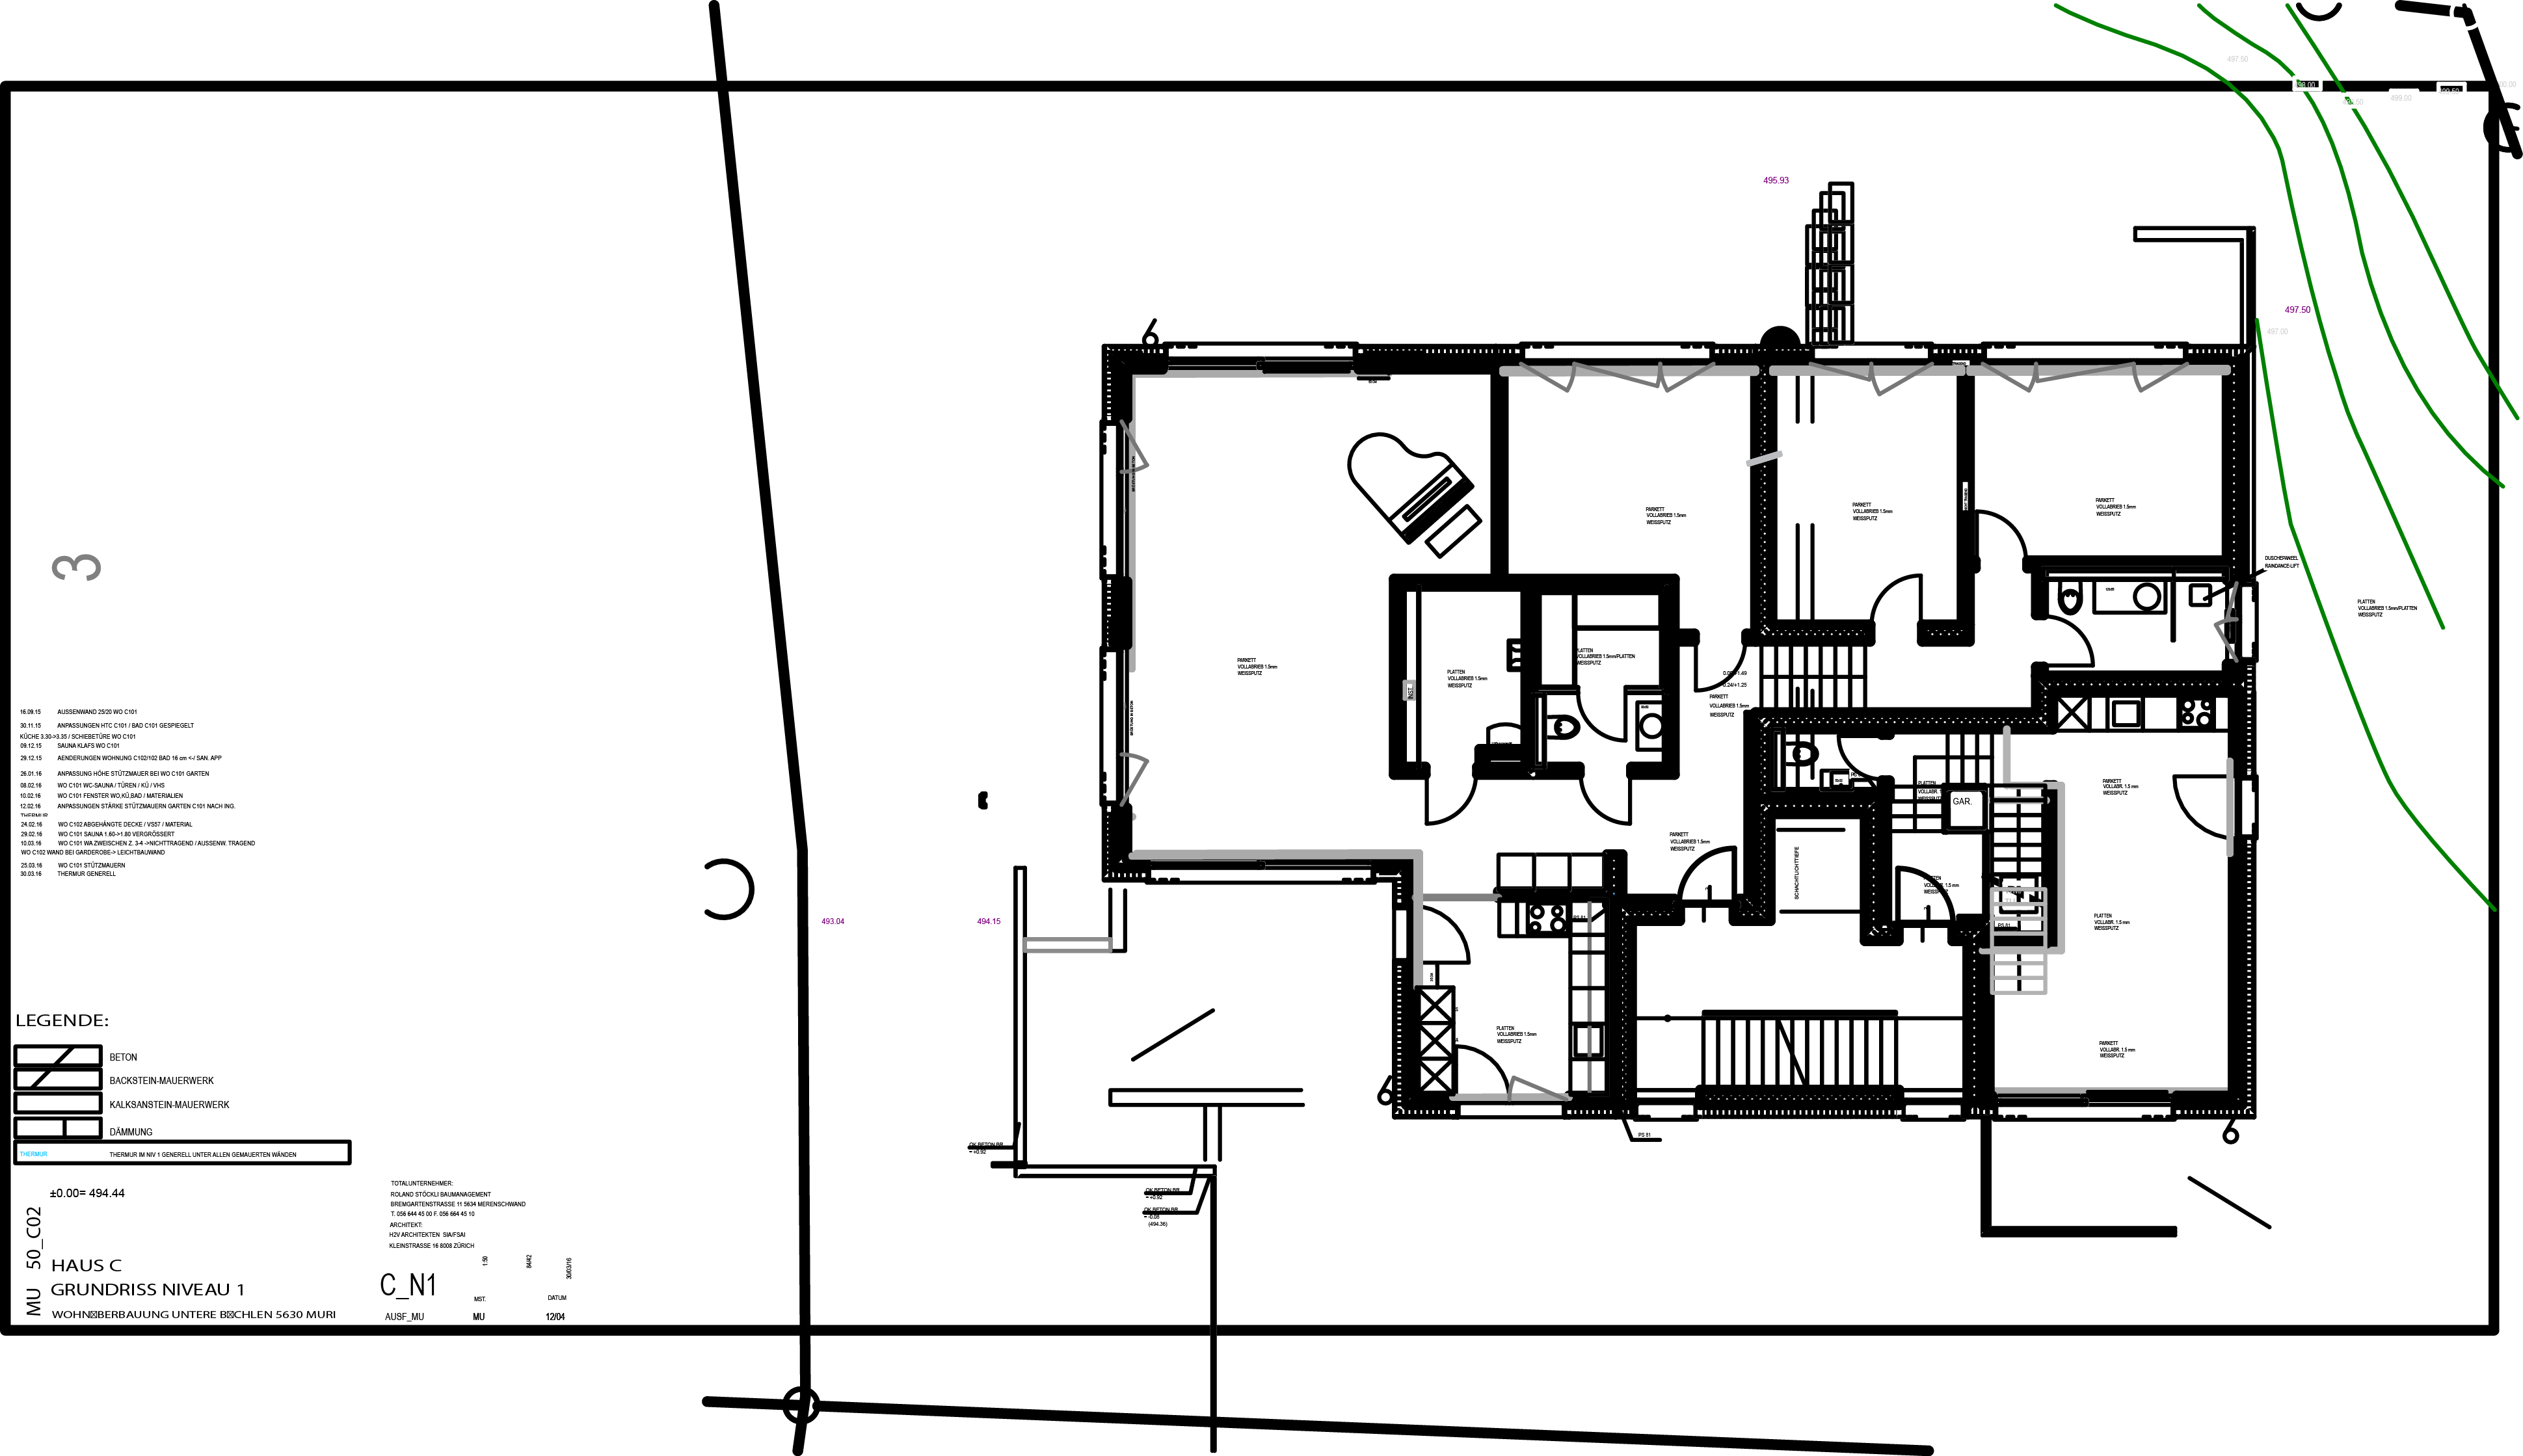
\includegraphics[width=0.4\textwidth]{A_N1.png}\label{fig:A_N1}}
	\hfill
	\subfloat[Image after noise removal.]{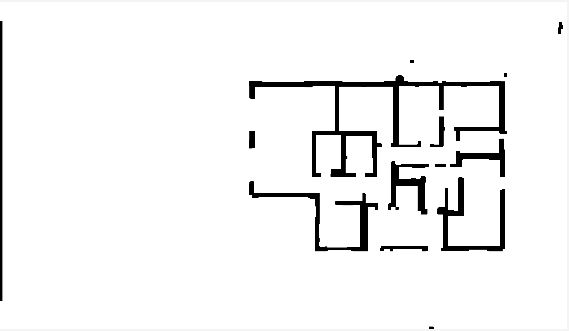
\includegraphics[width=0.4\textwidth]{morphtransuncleaned.jpg}\label{fig:A_N1_Morph}}
	\caption{Before and after of an uncleaned floor plan with noise removal. }
\end{figure}

\begin{figure}[h]
	\centering
	\subfloat[Original image.]{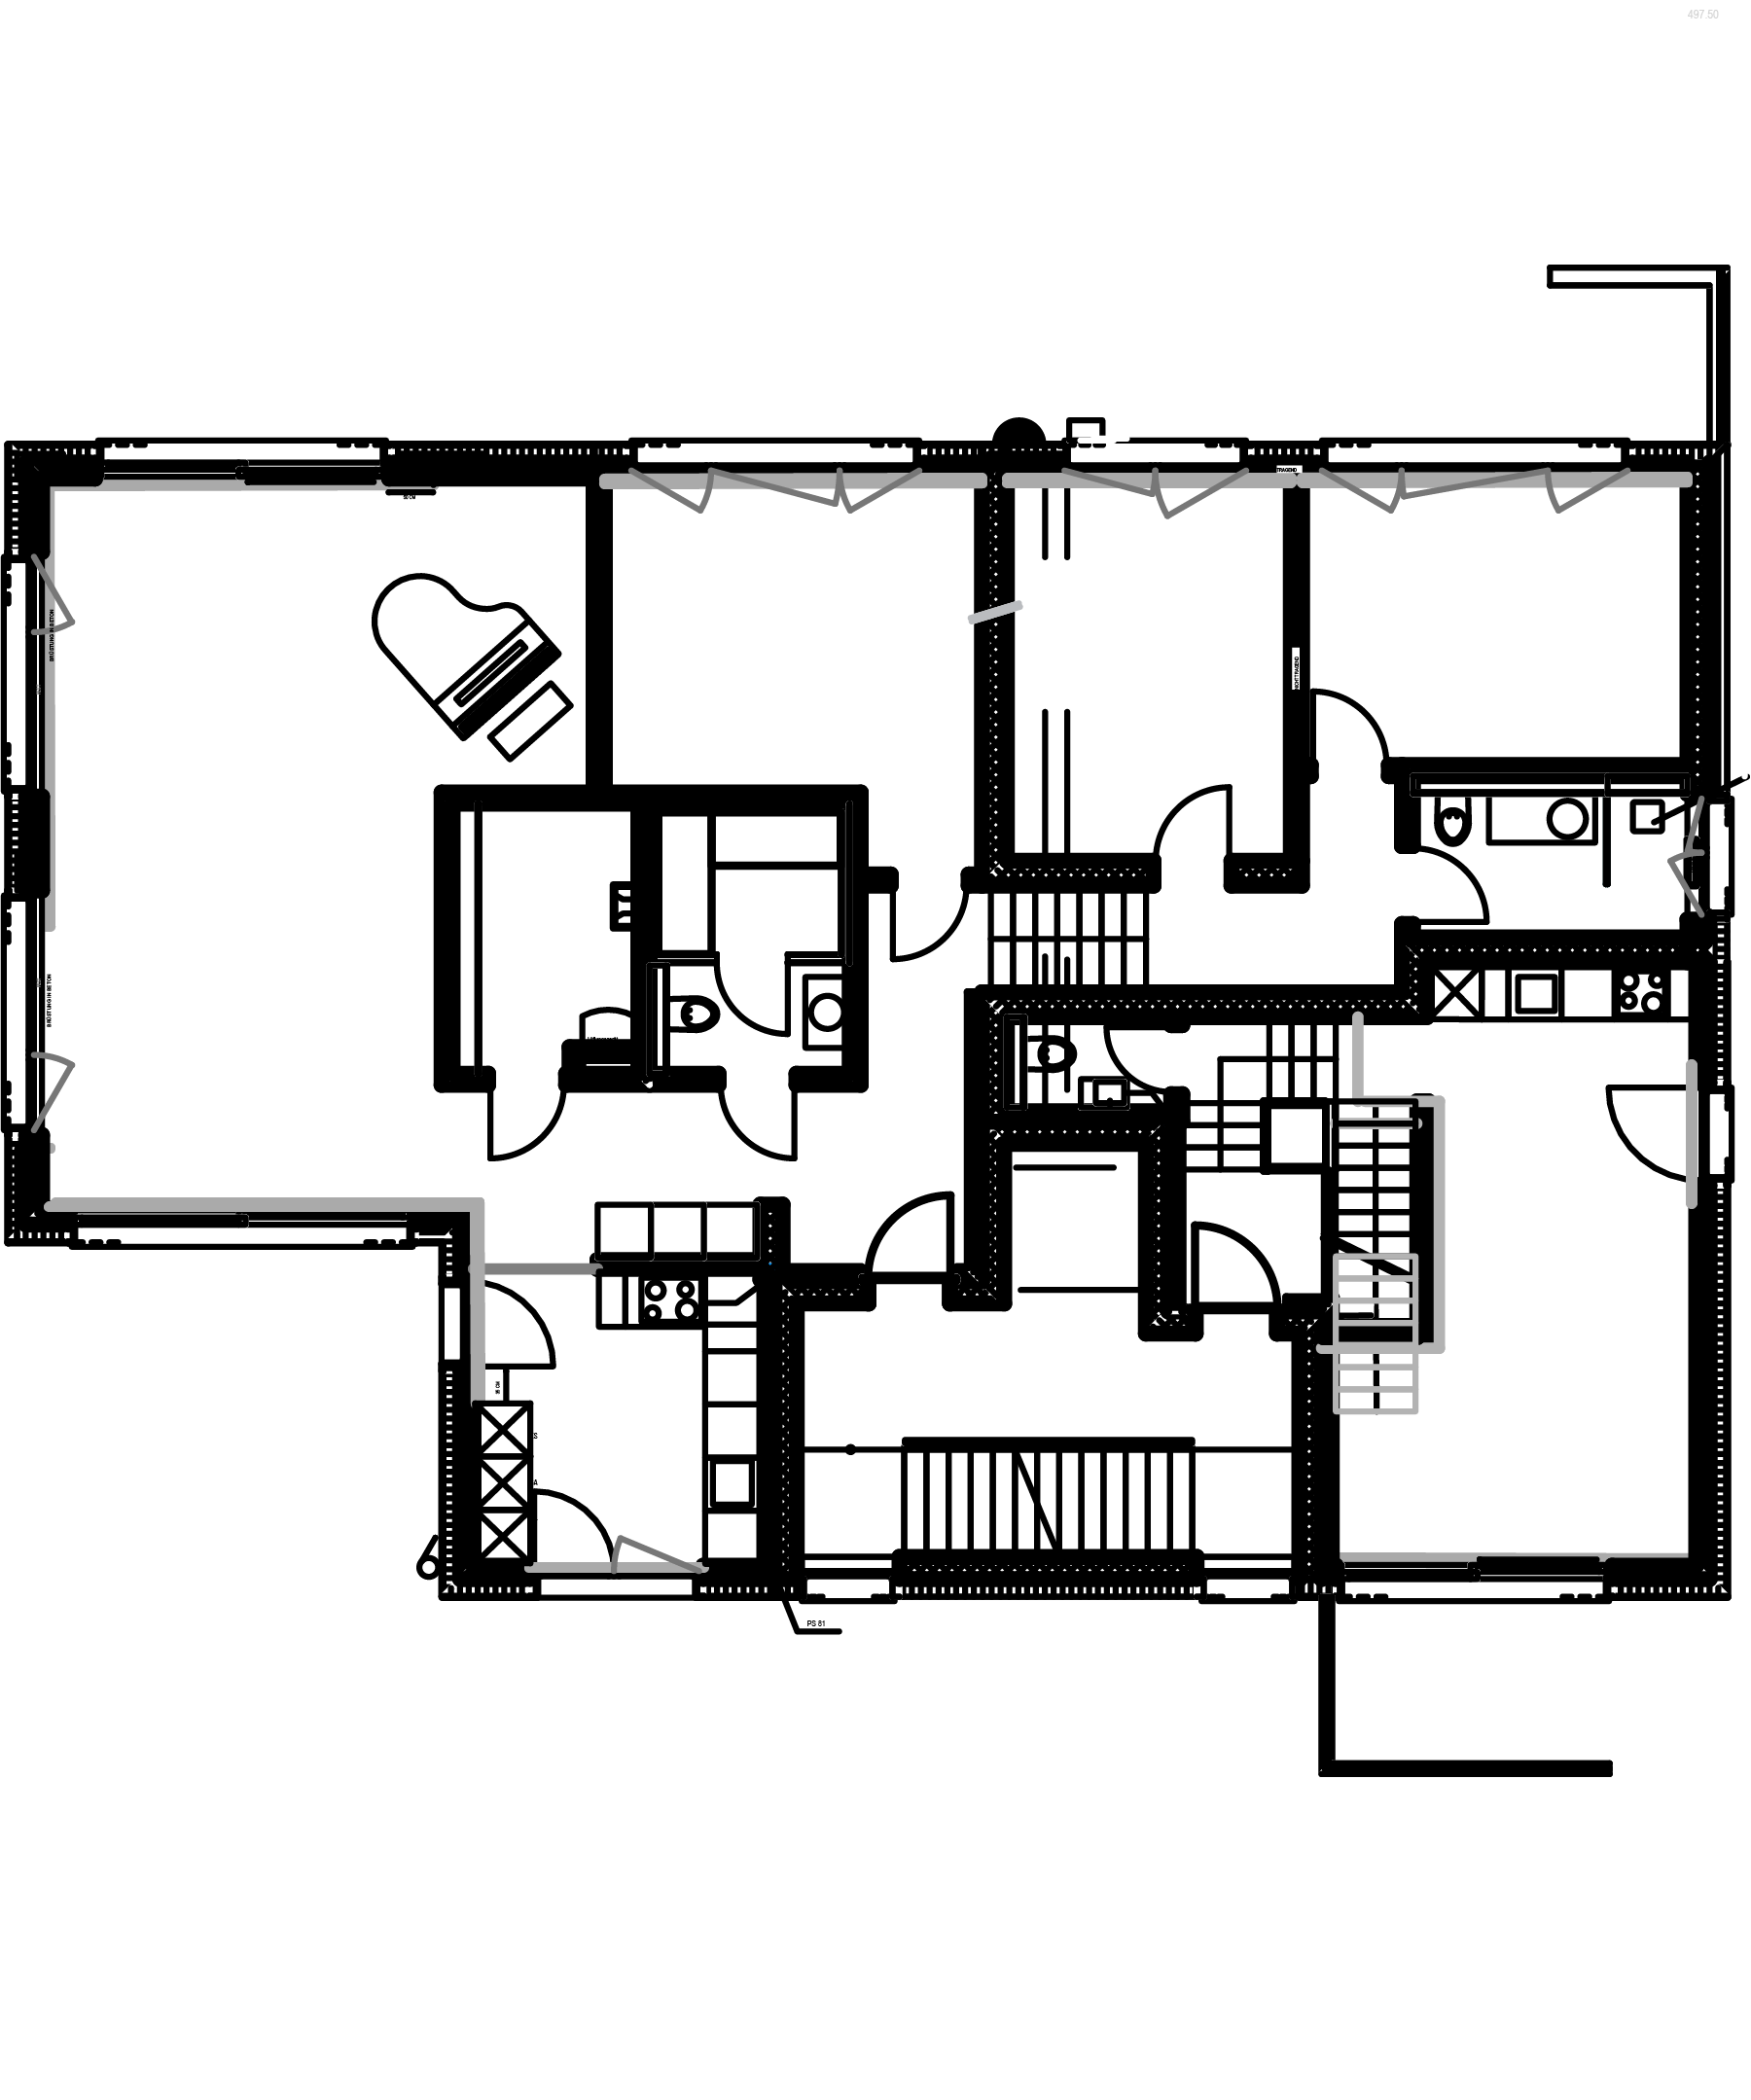
\includegraphics[width=0.4\textwidth]{A_N1_cleaned.png}\label{fig:A_N1_cleaned}}
	\hfill
	\subfloat[Image after noise removal.]{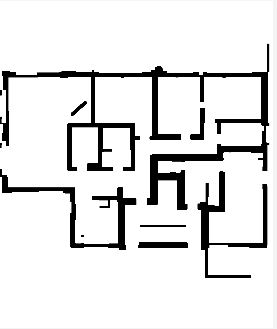
\includegraphics[width=0.4\textwidth]{morphtranscleaned.jpg}\label{fig:A_N1_cleaned_Morph}}
	\caption{Before and after of a cleaned floor plan with noise removal.}
\end{figure}

The figure~\ref{fig:A_N1} is one of the uncleaned testing images before any noise removal. It was cleaned up with an erosion/dilation size of 8. Figure~\ref{fig:A_N1_Morph} is the result of the noise removal. It is easily visible that most of what's left are walls. Due to the thin lines of the windows they get removed in the process. Those will be added later though as they are an important part of the wall to surround the rooms.

The same was done to the cleaned up image. As a result of different image sizes the noise removal was actually worse with the same parameters. This shows that each different image has very specific parameters for an optimal noise removal. This is further discussed in the section \ref{subsec:Parameter Finding}.

As this is not perfect due to the variety of possible objects on a plan, there is the option to delete those beforehand or afterwards with our built in editor. This is so we can manually improve the quality of the outcome of noise removal.

As a result of the noise removal we get an image with very basic information about where the walls are. This will be very important for our next step and other steps to come.

\todo{Discuss specific parameters for each image in parameter finding}
\todo{Distance Transform, Why not Contour Detection}

\subsection{Structural Analysis}
\todo{Object Detection: TM, Hough Lines, ORB}
\todo{Cascading Classifier: To few samples, Cat images prove, more positive, thickening, polydp, positive negative ratio, more specific negative samples}
\todo{Object Single Cases}
\todo{Gaps Closing: Clustering, Rotation / MinBox}

\subsection{Semantic Analysis}
\todo{Watershed}
\todo{Polygon Smoothing}